\section{Electromagnetic Waves}
Propagation of electromagnetic waves is described by the complete set of Maxwell equations either in frequency- or time domain. However, it is a common practice to derive and solve a single electromagnetic wave equation (E-field \textbf{or} H-field).\\

E-Field wave equations in time and frequency domain:
\begin{equation*}
	\Delta \vec{E} - \underbrace{\mu\sigma\frac{\partial \vec{E}}{\partial t}}_{\textrm{losses}} - \underbrace{\mu\varepsilon\frac{\partial^2 \vec{E}}{\partial t^2}}_{\textrm{wave}} = 0
	\hspace{2cm}
	\Delta \underline{\vec{E}} - j\omega\mu\sigma\underline{\vec{E}} + \omega^2\mu\varepsilon\underline{\vec{E}} = 0
\end{equation*}
H-Field wave equations in time and frequency domain:
\begin{equation*}
	\Delta\vec{H} - \underbrace{\mu\sigma\frac{\partial \vec{H}}{\partial t}}_{\textrm{losses}} - \underbrace{\mu\varphi\frac{\partial^2 \vec{H}}{\partial t^2}}_{\textrm{wave}} = 0
	\hspace{1.8cm}
	\Delta \underline{\vec{H}} - m\omega\mu\sigma\underline{\vec{H}} + \omega^2\mu\varepsilon\underline{\vec{H}} = 0
\end{equation*}

\textbf{\\ Boundary Value Problem (BVP)\\}
\begin{minipage}[lt]{11cm}
	\begin{tabular}{l}
		\(\displaystyle \vec{n} \times \vec{E} = 0, \textrm{ over }\partial_{\mathrm{PEC}}\Omega \) \\
		\(\displaystyle \vec{n}_1 \times \left(\nabla \times \vec{E}\right) + jk_z\vec{n}_1 \times \left(\vec{n}_1 \times \vec{E}\right) = \) \\
		\(\displaystyle \hspace{2cm}2jk_z \vec{n}_1 \times \left(\vec{n}_1 \times \vec{E}_i\right), \textrm{ over } \partial_{\mathrm{PORT1}}\Omega \) \\
		\(\displaystyle \vec{n}_2 \times \left(\nabla \times \vec{E}\right) + jk_0\vec{n}_2 \times \left(\vec{n}_2 \times \vec{E}\right) = 0, \textrm{ over } \partial_{\textrm{PORT2}}\Omega \) \\
		\(\displaystyle k_z = \sqrt{\omega^2\mu\varepsilon-k_t^2} \) \\
		\(\displaystyle k^2_{tmn} = \left(\frac{m\pi}{a}\right)^2 + \left(\frac{n\pi}{b}\right) ^2\) \\
	\end{tabular}
\end{minipage}
\begin{minipage}[rt]{8cm}
	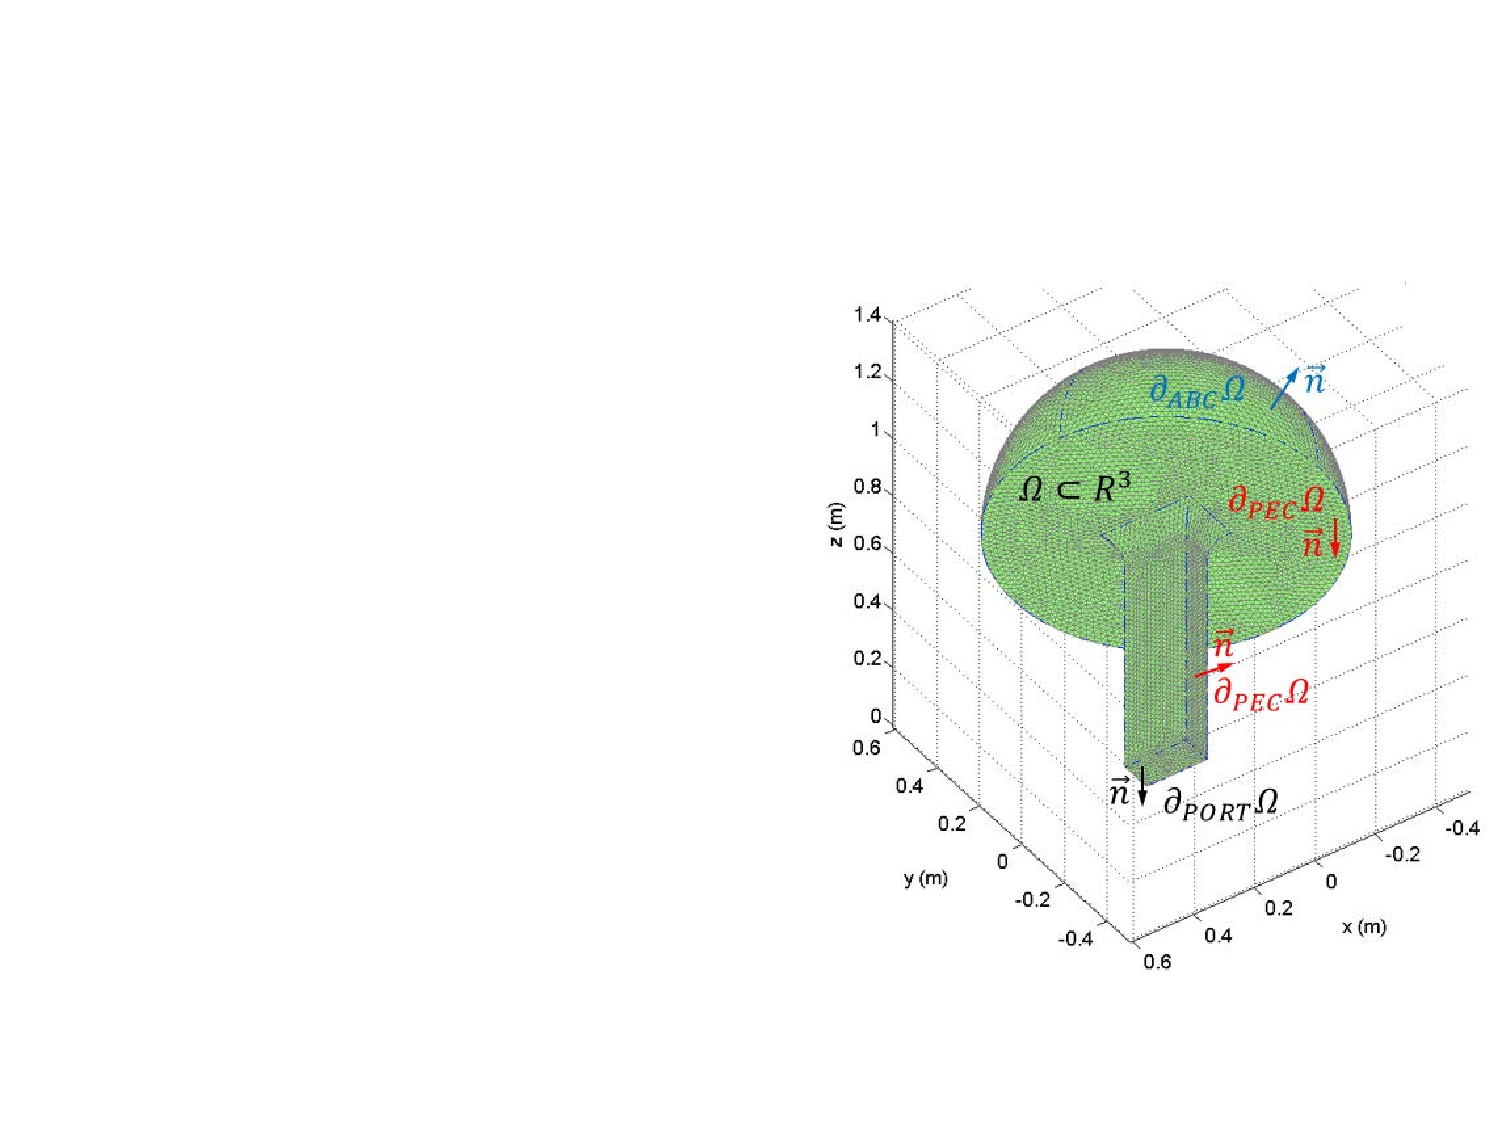
\includegraphics[width=.8\textwidth]{./images/BVP_wave.pdf}
\end{minipage}